\documentclass[runningheads,a4paper]{llncs}

\usepackage{amssymb}
\setcounter{tocdepth}{3}
\usepackage{graphicx}


\usepackage{graphicx}
\usepackage{caption}
\usepackage{subcaption}
\usepackage{float}
\usepackage[vlined,algoruled,titlenumbered,noend]{algorithm2e}
\usepackage{hyperref}
\usepackage{ctable}

\hypersetup{
	colorlinks   = true,
       linkcolor = red,
            urlcolor  = blue,
            citecolor = blue
}

\usepackage{url}
\urldef{\mailsa}\path|{email1,email2} |
\urldef{\mailsb}\path|anna.kramer, leonie.kunz, christine.reiss, nicole.sator,|
\urldef{\mailsc}\path|erika.siebert-cole, peter.strasser, lncs}@springer.com|    
\newcommand{\keywords}[1]{\par\addvspace\baselineskip
\noindent\keywordname\enspace\ignorespaces#1}

\usepackage{times}
\usepackage{helvet}
\usepackage{courier}

\usepackage{times}
\usepackage{latexsym}
\usepackage{amsmath}

\usepackage{amssymb}
\setcounter{tocdepth}{3}
\usepackage{graphicx}
\usepackage{subcaption}

\usepackage{amsmath}
\usepackage{graphicx}
\usepackage{caption}
\usepackage{subcaption}
\usepackage{float}
\usepackage[vlined,algoruled,titlenumbered,noend]{algorithm2e}
\usepackage{hyperref}
\usepackage{ctable}

\hypersetup{
	colorlinks   = true,
       linkcolor = red,
            urlcolor  = blue,
            citecolor = blue
}

\usepackage{url}
\DeclareMathOperator*{\argmax}{\arg\!\max}



\frenchspacing
\setlength{\pdfpagewidth}{8.5in}
\setlength{\pdfpageheight}{11in}

\setcounter{secnumdepth}{0}  

\begin{document}

\mainmatter  % start of an individual contribution

% first the title is needed
\title{Exploiting Structured Elements to improve Retrieval}

% a short form should be given in case it is too long for the running head
%\titlerunning{Lecture Notes in Computer Science: Authors' Instructions}

% the name(s) of the author(s) follow(s) next
%
% NB: Chinese authors should write their first names(s) in front of
% their surnames. This ensures that the names appear correctly in
% the running heads and the author index.
%
\author{Author 1%
\and Author 2 \and Author 3}
%
%\authorrunning{Lecture Notes in Computer Science: Authors' Instructions}
% (feature abused for this document to repeat the title also on left hand pages)

% the affiliations are given next; don't give your e-mail address
% unless you accept that it will be published
\institute{Institute1\\ Institute 2\\ Institute 3\\
\mailsa\\
}

%
% NB: a more complex sample for affiliations and the mapping to the
% corresponding authors can be found in the file "llncs.dem"
% (search for the string "\mainmatter" where a contribution starts).
% "llncs.dem" accompanies the document class "llncs.cls".
%

\toctitle{Lecture Notes in Computer Science}
\tocauthor{Authors' Instructions}
\maketitle
\begin{abstract}
Word embeddings have recently been shown to be effective in improving retrieval. 
However, existing word embeddings rely on plain text and do not take into consideration the 
structure of a web document which is traditionally a popular means of extracting 
features for query-document matching. The underlying assumption of existing word embeddings 
from plain text documents is that semantically related words occur together. However, 
these embeddings may not provide a succinct representation of web documents. Webpages provide  
a lot more meta-information about each word. We can extract multiple properties of a word such 
as its color, size or location in a webpage. Integration of these properties into existing word 
embeddings would yield a much richer representation of web documents which can be used to perform 
several tasks such as clustering, retrieval or spam detection. 

In this preliminary work, we exploit these structural properties to create 
richer embeddings for web documents. We specifically exploit location of words and structure 
of web page to create these embeddings. We evaluate the utility of these embeddings with retrieval. 
Our experiments show that structure embeddings clearly outperform plain text word embeddings 
on four years of Web track TREC corpus. 
\end{abstract}

\section{Introduction}
\label{sec:introduction}
% Retrieval is common
% Documents are becoming more and more complex with a lot of things in it beyond 
%textual content
% Why are embeddings popular % How are the built % How are they used in 
%information retrieval % What are the shortcomings of existing embeddings
% Importance of structure and our solution
% Research questions and findings
With exponential growth in digital content , an increasing number of users rely 
on search engines to find information on a daily basis. In order to assist users 
in finding the right information with least effort, search engines rely heavily 
on information retrieval. As opposed to the early days of 
internet when most web documents primarily comprised of textual content, modern 
day documents are inherently more complex and composed of heterogeneous 
structural elements including, but not limited to images, tables or entity 
panels.

Learning comprehensive representations of data is a critical component of any 
system that ranks documents. Classical retrieval models such as TF-IDF and BM25, 
use a bag-of-words representation and cannot effectively capture contextual 
information of a word. Researchers have also used vector representations of text 
that embed document and query text into a lower dimensional space using 
LSA\cite{deerwester1990indexing}, PCA\cite{jolliffe1986principal} 
or LDA\cite{blei2003latent} to compute query-document similarity. Several models are also 
trained with hand crafted features \cite{Cao2006Sigir,Burges2010Report,Chapelle2011Yahoo} 
that capture query specific syntactic or semantic information from the document. 
These features may rely on frequency, position or proximity of query terms in web documents. 
The above approaches have a major shortcoming: they either require manual decison on several 
hyperparameters (number of dimensions, topics or vectors) or manually 
designed features. Such approaches may not succinctly represent and exploit query 
or document information which may yield suboptimial rankers. 


With rapid progress 
in deep learning and distributional semantics, hand-crafted features are no 
longer required. Neural IR models can now exploit myriad types of large 
scale pre-trained vector representations to learn a high-dimensional scoring 
function for a query and document.
Recently proposed neural architectures \cite{zheng2015learning,zamani2016estimating,mitra2015query} 
rely on word embeddings that directly 
exploit word co-occurance. However, these embeddings do not 
directly capture the rich structural information available in web documents.  
Specifically, existing word embeddings fail to capture insights 
from the presence of and content embedded in structural elements of web pages 
which may limit the performance of existing rankers. 

Given the significant diversity in the content of web documents, 
in this preliminary study, we go beyond textual content and aim to leverage 
various heterogeneous structural elements in a web document to create richer embeddings. 
% \textcolor{red}{TODO: add 1-2 lines on 
% past papers which support our structured elements claims.} 
From a relevance and user satisfaction perspective, we hypothesize that users 
often spend less cognitive effort in finding information in structured 
tables or entity panels than in reading through multiple paragraphs in a webpage. 
Given the importance of structural elements in webpages and their absence from 
existing embeddings, we posit that training rankers that jointly exploit 
distributional semantics and word level meta-data will perform better than 
traditional models. 

In this work, we undertake the task of learning richer document representations 
and propose a novel neural ranking architecture that exploits both co-occurance and 
structural information associated with every word in the web page. 
We begin by investigating document composition of TREC Web documents to 
understand the distribution of structural elements in web corpus. Specifically, we consider four different 
types of structural elements: (i) images, (ii) tables, (iii) headings, (iv) lists and (v) hyperlinks to 
understand the interplay between the presence of such elements and document relevance. 
We propose a neural architecture which jointly exploits structural element embedding and 
word embeddings to rank documents.

Given the rich representations of documents, we perform preliminary experiments to 
demonstrate the efficacy of the proposed model. We observed 
slight but statistical improvements in NDCG over existing baselines. This indicates the 
advantage of exploiting underlying structure of web pages in retrieval. We posit that proposed 
architecture, when augmented with more refined information about a webpage would significantly 
improve retrieval accuracy. In future, we aim to experiment with recurrent networks that directly 
exploit word or character level information to reduce proposed model's dependency on 
pre-trained word embeddings.





\section{Related Work}
\label{sec:related_work}
Our work spans multiple areas of research. We review literature that addresses 
construction of word embeddings and their utility in information retrieval.
\begin{figure}[t]
        \centering
%        \includegraphics[width=\linewidth]{elements.pdf}
        \caption{Percentage distribution of the presence of different structural 
elements considered.}
        \label{fig:elements}
\end{figure}
\subsection{Distributional Semantics for IR}
While many word embedding models have been proposed recently, the Continuous 
Bag-of-Words (CBOW) and the Skip-Gram
(SG) architectures proposed by Mikolov et al. \cite{mikolov2013distributed} are 
arguably the most popular. More recently, a theoretical framework was proposed 
which estimates query embedding vectors based on the individual embedding 
vectors of vocabulary terms \cite{zamani2016estimating}. In terms of 
applications, word embeddings have been studied in various IR contexts such as 
term reweighing \cite{zheng2015learning}, cross-lingual retrieval 
\cite{vulic2015monolingual} and short text similarity 
\cite{kenter2015short}. Beyond word co-occurrence, recent studies have also 
explored learning text embeddings from click-through data 
\cite{shen2014learning}, session data \cite{grbovic2015context} and for query 
prefix-suffix pairs \cite{mitra2015query}. Finally, Diaz \textit{et al.} 
\cite{diaz2016query} highlight the value of locally-training word embeddings retrieval. 
We explore the use of embeddings to represent 
contributions from different structural elements comprising document and 
proposing novel ways of leveraging such representations for improved document 
retrieval.

%\subsection{Document Retrieval with embeddings}
\subsection{Document Representations}
Vector based representation of documents is a standard practice in retrieval. 
A document vector simply encapsulates the importance of each 
term in the document and is usually highly dimensional. As a consequence, 
these vectors are sparse. To address the data
sparsity issue, several dimensionality reduction approaches have been proposed 
in the literature. A popular class of
methods is based on linear projection, which projects a high-dimensional vector on to a lower dimensional space. 
A historical approach to linear projection is Principal Component Analysis (PCA) 
\cite{jolliffe1986principal}, which performs a singular value decomposition 
(SVD) on a document matrix D of size n $\times$ m, where each row in D is the 
term vector representation of a document. Latent Semantic Analysis (LSA) 
\cite{deerwester1990indexing} is very similar to PCA but performs the SVD using 
the correlation matrix instead of the covariance matrix, which implies a lower 
computational cost. Other projection models such as Latent Dirichlet Allocation 
(LDA) \cite{blei2003latent} are based on the generative models of text in documents. 
Another approach, named Explicit Semantic Analysis (ESA) 
\cite{gabrilovich2007computing}, represents each document by its similarities to other documents in a collection. 
Using a low domain specificity document collection such 
as Wikipedia, the model has proven to obtain competitive results. Deep 
architectures have been shown to be highly effective in discovering from 
training data the hidden structures and features at different levels of 
abstraction useful for a variety of tasks. Liu \textit{et al.} 
\cite{liu2015representation} propose a representation Learning technique which 
makes use of a Multi-Task Deep Neural Networks for semantic retrieval. Recently, 
Shen \textit{et al.} \cite{shen2014learning} present a series of new latent 
semantic models based on a convolutional neural network (CNN) to learn 
low-dimensional semantic vectors for search queries and Web documents. The 
interested reader is directed to Li \textit{et al.} \cite{li2014semantic} which 
presents a comprehensible survey summarizing different semantic matching 
techniques.
\begin{figure*}[t]
        \centering
        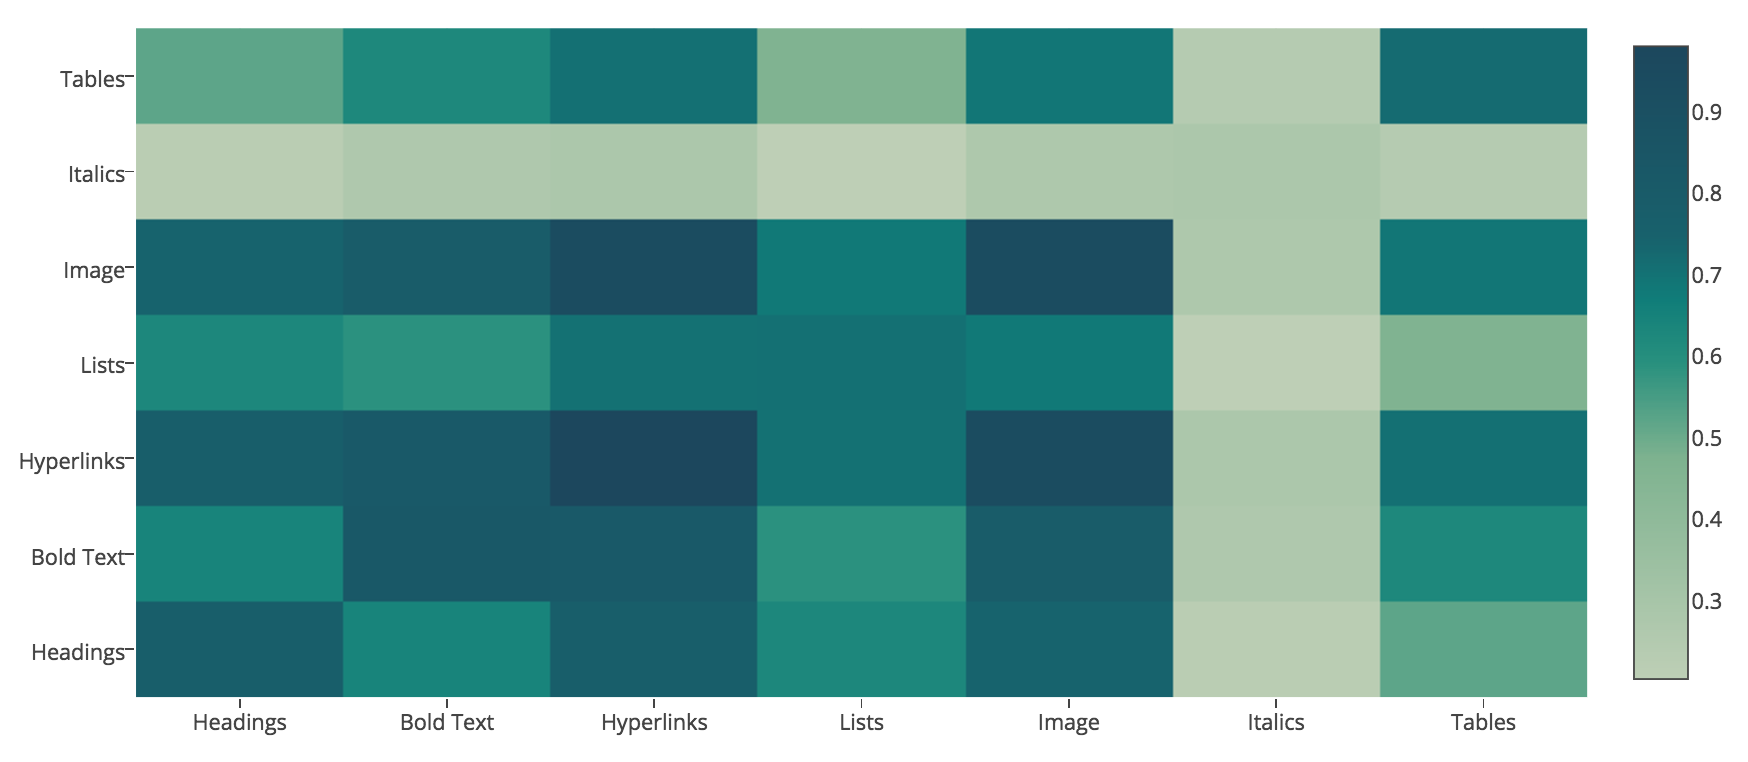
\includegraphics[width=0.8\linewidth]{heatmap.png}
        \caption{Element co-occurrence visualized via heatmap.}
        \label{fig:heatmap}
\end{figure*}
\subsection{Exploiting Document Structure}
Beyond exact and semantic matching of queries and documents for retrieval, the 
use of number of different features and elements have been explored by enhanced 
retrieval techniques. Tombros \textit{et al.} \cite{tombros2005users} 
investigate the criteria used by online searchers  and presented the relative 
utility of features: web page content,
structure and quality and their importance when assessing the relevance of web 
pages for information-seeking tasks. Hui \textit{et al.}\cite{hui2017position} 
consider positional information and propose position-aware representations for 
relevance matching in a neural retrieval framework. Recently  \cite{verma2016obtaining} 
found that presence of structural elements in webpage reduce user's overhead in finding 
required information from a webpage quickly which provides a strong motivation for our work 





\section{Methodology}
\label{sec:methodology}
We begin with brief overview of elements used in this work to generate structural embeddings. 
This is followed by a detailed overview of the model used to jointly score documents and train 
structure embeddings. We compare the performance of the proposed architecture with some 
state-of-the-art learning to rank models. Finally, we provide a short description of the 
datasets and evaluation metrics used in this work.
\subsection{Structural Elements}
Web pages comprise of several structural elements. However, in this work we primarily study 
role of a small subset of structural elements in a webpage. We consider seven elements 
listed below.
\begin{enumerate}
\item \textbf{Headings:} Human beings use document or section headings as anchors 
or entry points \cite{} to paragraphs. Often headings summarize information conveyed by 
the text in the forthcoming paragraph, and can be treated as a separate element. 
\item \textbf{Tables:} The presence and contents of any tabular data in the 
document (table layout) is categorized in the Tables element. Certain type of 
information e.g. statistics, are easy to find in a table than scanning an  
entire document. In this work, we consider entire content in a table for learning 
its low-dimensional representation.
\item \textbf{Bold and Italics:} Any italicized or bold text is treated as a separate element. Often 
certain phrases are marked in bold text to convey their importance. 
All bold textual content is treated as a separate element.
\item \textbf{Hyperlinks:} Any reference to data (within the same document or 
across different web documents) that the reader can directly follow either by 
clicking, tapping, or hovering is considered as a hyperlink. We consider the 
anchor text of all hyperlinks present in a document under this element.
\item \textbf{Lists:} Authors often create ordered or unordered lists of content to summarize key points 
which in turn makes it easier for readers to parse information quickly. All textual 
content present in such lists is considered under the Lists structural element.
\item \textbf{Images:} Information items that are of a non-textual form, i.e., 
pictures or GIFs or videos comprise the Images entity category. In this work, we use meta-data 
contained in the image element to create embeddings. 
\end{enumerate}

It is important to analyze how these elements are distributed in a web corpus 
to approximate the quality of embeddings. Sparsely distributed elements that contain 
less textual content may not yield useful representations. Thus, we 
first analyze the distribution of above listed elements in Clueweb corpus labeled in 
TREC Web track 2011-2014. 
Figure \ref{fig:elements} presents the distribution of each of the seven 
structural elements listed above. We observe that hyperlinks and images are most 
common with over 90\% web documents containing at least one hyperlink or image. 
Specialized formats such as tables and lists are found in over 70\% of web 
documents.

In terms of formatting of textual content, bold texts and headings 
are much more commonly found in documents than italicized text, with less than 
30\% documents containing italicized text. In addition to the popularity of each 
element (Figure \ref{fig:elements}), we also look at the element co-occurrence 
patterns using a heatmap of co-occurring elements in Figure 
\ref{fig:heatmap}. We observe that Images are accompanied more by Hyperlinks in 
web documents than by Tables. Overall our analysis indicates myriad usage of 
structural elements in web documents in clueweb corpus. This re-emphasizes that 
these elements, if exploited, may indeed be useful in retrieval.  
% \textcolor{red}{TODO: did we normalize the values 
% per element? everything seems to go well with Hyperlinks! :P}
% \textcolor{green}{Per element? Its just $\frac{\sum 1(ele1)  \cap  
% 1(ele2)}{total_d}$ where $1(x)$ indicates whether x is present in d.}
    \begin{figure*}
    \centering
    \caption{Network architecture}
    \label{fig:network_architecture}
    \begin{subfigure}[b]{0.70\textwidth}
    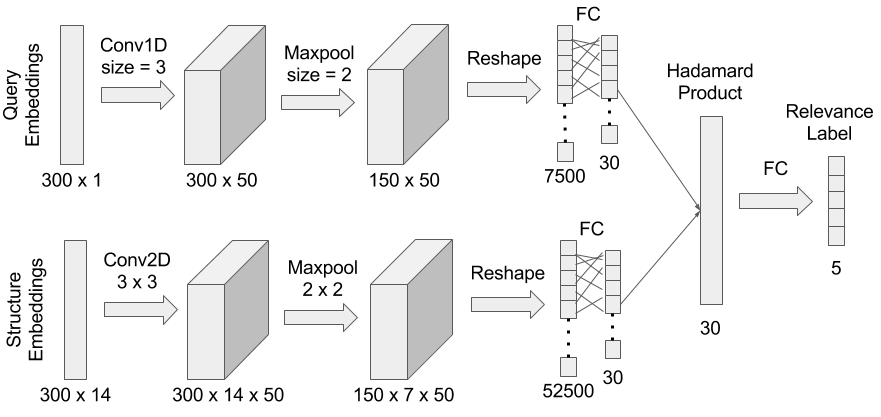
\includegraphics[width=\textwidth]{diagrams.png}
    \end{subfigure}
    \end{figure*}
\subsection{Retrieval with structure embeddings}
For preliminary analysis we rely on a simple convolutional neural 
network architecture that predicts both relevance of a document with 
respect to a search query and its structural embedding. 
The network architecture with each layer, input and output size 
is given in Figure \ref{fig:network_architecture}. 
Given $\mathit{Q}$ queries, $\mathit{D}$ documents in corpus and $\mathit{S}$ 
structural elements in a webpage, the model projects a query 
and document into an embedding space before scoring.

The proposed network has two input vectors: query and document. We represent each 
query $q_i \in \mathit{Q}$ query with 300\footnote{300 dimensional 
embeddings are standard in practice 
\cite{mitra2015query,zamani2016estimating}} dimensional vector. 
In this experiment, we represent each document $d_j \in \mathit{D}$  
with a stacked two-dimensional matrix, where each row is the embedding 
of $s_k \in \mathit{S}$ structural element. 
\begin{table}
  \centering
 \caption{Query and label distribution of 2011-2014 Web track}
 \label{table:data_distribution} 
 \begin{tabular}{|c|c|c|c|}
\hline
Year	&	\#q	&	\#docs	&	\#rel	 \\ \hline
2011	&	50	&	19381	&	3157		\\ \hline
2012	&	50	&	16102	&	3523		\\ \hline
2013	&	50	&	14531	&	4149		\\ \hline
2014	&	50	&	14610	&	5665		\\ \hline
 \end{tabular}
\end{table}

Each query vector is first passed through one-dimensional convolutional
layer with 50 filters, kernel size of 3 and stride of 1. 
However, each document vector is first passed through a two-dimensional convolutional
layer with 50 filters, a kernel size of 3X3, and a stride of 1. 

While, output of query convolution layer is further passed into a size 2 pooling 
layer, output of document convolution layer is passed into size 2x2 pooling layer.  
This is followed by reshaping and a final fully-connected layer 
that produces a single real-valued vector. 
All the nodes in the model use the rectified linear unit (relu) function 
for non-linearity.

\begin{table*}
 \caption {$NDCG@$1 and $NDCG@$10 for 2011-2014 }
 \label{table:network_perf} 
 \begin{tabular}{|c||c|c|c|c||c|c|c|c|} \hline
& \multicolumn{4}{|c|}{NDCG@1} &  \multicolumn{4}{|c|}{NDCG@10} \\ \hline
System &  2011 & 2012  & 2013 & 2014 &  2011 & 2012  & 2013 & 2014 \\ \hline
$SVM_r$ & \textbf{0.25} & \textbf{0.16} & 0.23 & 0.17 & \textbf{0.26} & 0.13 & 0.27 & 0.23   \\
$LMart$ & 0.23 & 0.10 & 0.22 & \textbf{0.27} & 0.24 & \textbf{0.16} & 0.30 & \textbf{0.29} \\
$SEmbed_{all}$   & 0.21$^\downdownarrows$ & 0.11$^\downdownarrows$ & \textbf{0.24$^*$}  & 0.25$^\upuparrows$ & \textbf{0.26} & 0.15$^*$ & \textbf{0.32}$^\upuparrows$ & \textbf{0.29}$^\upuparrows$\\ \hline 
$SEmbed_{head}$  & 0.05 & \textbf{0.10}$^\downdownarrows$ & \textbf{0.16}$^\downdownarrows$ & 0.13$^\downdownarrows$ & 0.08$^\downdownarrows$ & \textbf{0.14}$^\downdownarrows$ & \textbf{0.17}$^\downdownarrows$ & 0.16$^\downdownarrows$ \\ 
$SEmbed_{table}$ & \textbf{0.08}& 0.05$^\downdownarrows$& 0.09$^\downdownarrows$ & 0.13$^\downdownarrows$ & 0.07$^\downdownarrows$ & 0.09$^\downdownarrows$ & 0.14$^\downdownarrows$ & 0.19$^\downdownarrows$ \\
$SEmbed_{link}$  & 0.06& 0.05$^\downdownarrows$& 0.12$^\downdownarrows$& \textbf{0.24}$^\upuparrows$ & \textbf{0.10}$^\downdownarrows$ & 0.10$^\downdownarrows$ & 0.15$^\downdownarrows$ & \textbf{0.21}$^\downdownarrows$  \\ 
$SEmbed_{list}$  & 0.05& 0.05$^\downdownarrows$& 0.10$^\downdownarrows$ & 0.14$^\downdownarrows$ & 0.09$^\downdownarrows$ & 0.11$^\downdownarrows$ & 0.15$^\downdownarrows$ & 0.17$^\downdownarrows$\\ 
$SEmbed_{img}$   & 0.03& 0.05$^\downdownarrows$& 0.13$^\downdownarrows$& 0.15$^\downdownarrows$ & 0.08$^\downdownarrows$ & 0.10$^\downdownarrows$ & 0.16$^\downdownarrows$ & 0.20$^\downdownarrows$ \\ \hline
\end{tabular}
\\
\footnotemark{p-val: $^*$ $\le$ 0.05,  $^\upuparrows$ $\le$ 0.001, $^\downdownarrows$ $\le$ 0.001 over SVMRank with paired t-test}
 \end{table*}
We compute the posterior probability of document relevance given a query 
from the semantic relevance score between them
through a softmax function in Equation \ref{eq:activation}. 
\begin{equation}
\label{eq:activation}
  p(R_{d_j} = r|q_i) = \frac{e^{\beta_r * f(q_i, d_j)}} {\sum_{0<c<K}e^{\beta_c * f(q_i, d_j)}}
\end{equation}

where $P(R_{d_j}=r|q_i)$ is the probability that relevance grade $R_{d_j}$ of 
document $d_j$ for query $q_i$ is $r$. $K$ represents different 
relevance grades in training data.

Given $M$ query, document pair and corresponding relevance label as 
training data, we optimize the cross-entropy loss 
function in Equation \ref{eq:loss_func}. 
\begin{equation}
 \label{eq:loss_func}
 \mathcal{L}(x;\theta) = - \frac{1}{n} \sum_{0<n<M}\sum_{0<c<K} 
    [ r_j ln ( \hat r_j) + (1 -  r_j)ln(1 - \hat r_j)]
\end{equation}
where $r_j$ and $\hat r_j$ are actual and predicted relevance labels of a document 
for a query respectively. $K$ represents different relevance grades in training data. 

We generate initial query and document embeddings using 
glove\footnote{https://nlp.stanford.edu/projects/glove/}. We generate embedding for each 
query by computing the average of its term embeddings. We create two dimensional 
document embeddings by stacking average term embeddings of the seven structural elements
listed above. 

The output of fully connected layer just after reshaping layer in Figure \ref{fig:network_architecture} 
would represent low dimensional structure embeddings for each document. 
Thus, in future, we shall investigate the utility of these embeddings for 
tasks other than retrieval. 

\subsection{Dataset}
We rely on TREC Web collection (2011-2014) \cite{collins2015trec} for 
our experiments. Table \ref{table:data_distribution} shows the distribution of 
relevance labels per year. 

We use 3 TREC Web datasets (150 queries)\footnote{Further divided into 4:1 
ratio for training and validation sets} to train and one dataset (50 queries) to test 
its effectiveness. For example, results for 2014 TREC web queries are obtained 
by training on 2011-2013 TREC web queries as training data. 

\subsection{Baselines}
Several algorithms exist
in the literature that optimize for relevance. In recent years, learning-to-rank 
approaches such as RankSVM \cite{Cao2006Sigir} and LambdaMart 
\cite{Burges2010Report} have proved to be effective in optimizing metrics such 
as NDCG. Thus, in this work we  compare the proposed model with both SVMRank and 
LambdaMart. 

LambdaMart \cite{Burges2010Report}  (\textbf{LMart}) relies on boosted 
regression trees to optimize non-smooth IR metrics such as NDCG. It has been 
extensively used in ranking tasks and also won Yahoo! Learning to rank 
challenge \cite{Chapelle2011Yahoo} in 2010. 
SVMRank \cite{Cao2006Sigir} ({$\boldsymbol{SVM_r}$}), a pairwise max-margin 
approach is used to learn a function to rank documents for a query. Given a set 
of document labels, query and document feature vectors, 
SVMRank optimizes the objective function learns a hyperplane that 
enforces ordering among relevant and non-relevant documents. 

Above approaches require hand-crafted features. We rely on features used in 
Letor \cite{liu2007letor}, a popular dataset which consists of several query, document text 
and structure specific features. For this preliminary work, we computed 68 
features to train and test these models.

\subsection{Evaluation metric}
\label{sec:evaluation}
There are several metrics that can be used to evaluate effectiveness of an IR 
system. 
In this work we rely on Normalized Discounted Cumulative Gain (NDCG) 
\cite{Jarvelin2000NDCG} 
to evaluate different systems. NDCG score at position $n$ is calculated as 
follows: 
\begin{equation}
 NDCG@n = Z_n \sum_{j=1}{n} \frac{2^{y_j} - 1}{log_2 j + 1}
\end{equation}
where $j$ is the position in the document list, $y_j$ is the label (relevance or 
effort) of 
the document $d_j$ in the list and $Z_n$ is the normalization factor which is 
the oracle 
discounted cumulative gain at position $n$ so that a perfect list gets NDCG 
score of 1.


\section{Results and Discussion}
\label{sec:results_and_discussion}
The performance of the proposed model is given in Table \ref{table:network_perf}. 
We report NDCG$@$1 and NDCG$@$10 for preliminary analysis. We also train and compare 
performance of model trained on each structural element. In this work, we compare 
models trained on headings ($SEmbed_{head}$), tables ($SEmbed_{table}$), 
lists ($SEmbed_{list}$), images ($SEmbed_{img}$) and hyperlinks ($SEmbed_{link}$). 

The proposed network architecture ($SEmbed_{all}$) performs significantly better than 
SVMRank trained on letor based features 
on three datasets (2012-2014). Statistical significance was computed using a paired t-test. 
These improvements suggest the importance of structural elements in web search. 
We posit that proposed architecture infers important features for each structure element automatically 
which is captured manually in features used in SVMRank or LambdaMart. 
An interesting exploration in the future would be to train and evaluate existing 
learning-to-rank models with pre-computed embeddings learnt via $SEmbed_{all}$.

We also trained a single network for each structural element to investigate  
its relative importance in retrieving relevant documents. It is expected that 
individual structural element will not perform better than model trained on 
combination of all elements. All structural models ($SEmbed_{head}$ - $SEmbed_{img}$) 
perform significantly lower than SVMRank baseline. 
However, their performance on all datasets shows that headings are the most useful amongst 
all other elements in retrieving relevant documents. On all datasets, 
$SEmbed_{head}$ performs better other models. 
This is followed by outlinks ($SEmbed_{link}$) and images ($SEmbed_{img}$) respectively. 
Tables ($SEmbed_{table}$) and lists ($SEmbed_{list}$), however, are not as useful as we had expected.
In future, we shall investigate the differences in embeddings of each element 
to understand their behaviour and impact on query-document matching in greater depth. 




\section{Conclusion}
\label{sec:conclusion}
Word embeddings have become a popular means to represent textual information in low-dimensional space. 
Several models have been proposed recently that exploit these embeddings to train neural architectures 
that perform significantly better than traditional models that relied on manually coded features. 
We argue that models based on word embeddings ignore a key aspect of web documents i.e. their structure. 
Each word in a web page can also be represented using its structural meta-data such as its location, size or 
style in webpage. Existing deep models do not encode structural information in a webpage in any form which 
traditionally has been used extensively to design query or document specific features. 

In this work, we tried to address the above shortcoming of existing models by proposing a simple 
neural framework that also encodes structural information of web page text to perform query-document matching. 
Our network takes query and document vectors (along with structure information) as input to predict document 
relevance. Preliminary experiments show that our approach performs better than existing learning-to-rank models 
trained on hand crafted features. We posit that our model automatically learns important textual 
and structural features to score a document against a search query. In future it would be worth 
investigating whether structural embeddings would be useful in tasks such 
as webpage clustering 
or classification.





\bibliographystyle{abbrv}
\scriptsize
{
\bibliography{sigproc-ECIR}
}


\end{document}



